%! Author = zero
%! Date = 29/07/2024

% Preamble
\documentclass[a4paper, 12pt]{article}

\usepackage[english,russian]{babel}
\usepackage[T2A]{fontenc}
\usepackage[utf8]{inputenc}
\usepackage{geometry}
\usepackage{enumitem}
\usepackage{setspace}
\usepackage{amssymb}
\usepackage{graphicx}
\usepackage{float}
\usepackage{wrapfig}
\geometry{top=5mm}
\renewcommand{\arraystretch}{1.2}
\linespread{1}

% Document
\begin{document}
    \begin{center}
        \textbf{Контрольная работа}
    \end{center}

    \begin{center}
        \textbf{№1 Переписать в символьном виде и посчитать}
    \end{center}

    \begin{enumerate}
        \item $A \wedge \bar B = 1 \wedge 1 = 1$
        \item $A \vee B = 1 \vee 0 = 1$
        \item $A \vee \bar B = 0 \vee 1 = 1$
        \item $A \wedge B = x \wedge 0 = 0$
    \end{enumerate}

    \begin{center}
        \textbf{№2 Решить кругами Эйлера}
    \end{center}

    \begin{minipage}[t]{0.4\textwidth}
        \centering
        \begin{enumerate}
            \item $A \wedge B$\\
            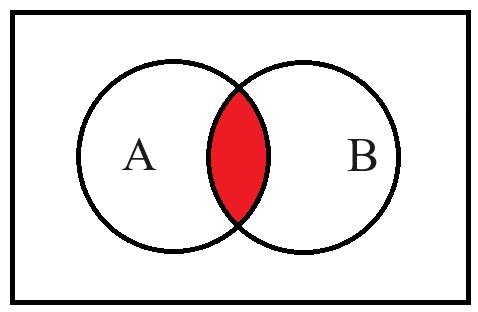
\includegraphics[width=1\linewidth]{images/img_2}

            \item $A \wedge \bar B \vee C$\\
            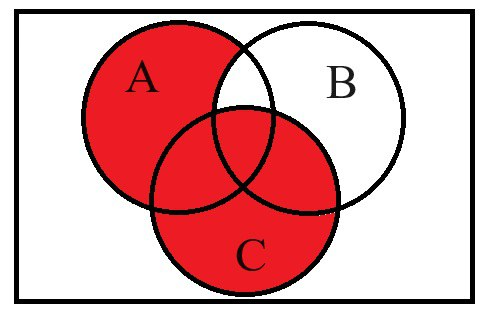
\includegraphics[width=1\linewidth]{images/img_3}
        \end{enumerate}
    \end{minipage}
    \begin{minipage}[t]{0.4\textwidth}
        \centering
        \begin{enumerate}
            \setcounter{enumi}{2}
            \item $\bar A \vee B \wedge C \vee D$\\
            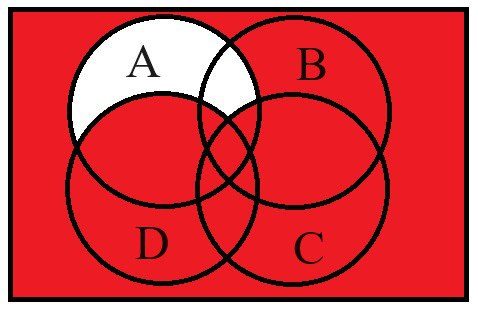
\includegraphics[width=1\linewidth]{images/img_4}

            \item $A \wedge B \vee C \wedge D$\\
            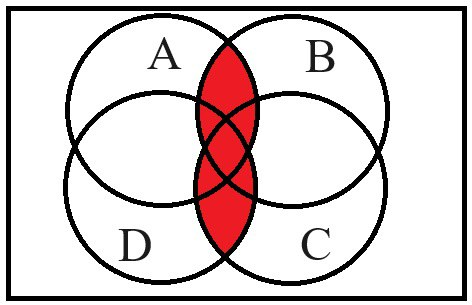
\includegraphics[width=1\linewidth]{images/img_5}

        \end{enumerate}
    \end{minipage}

    \begin{center}
        \textbf{№3 Построить таблицу истинности}
    \end{center}

    \begin{minipage}[t]{0.25\textwidth}
        \begin{enumerate}
            \setcounter{enumi}{0}
            \item \begin{spacing}{0.4}
                      $A \wedge \bar B$\\
            \end{spacing}
            \begin{tabular}{|x|y|f|}
                \hline
                $\textbf{A}$ & $\textbf{B}$ & $\textbf{f}$ \\
                \hline
                \hline
                0            & 0            & 0            \\
                \hline
                0            & 1            & 0            \\
                \hline
                1            & 0            & 1            \\
                \hline
                1            & 1            & 0            \\
                \hline
            \end{tabular}
            \setcounter{enumi}{2}
            \item \begin{spacing}{0.4}
                      $A \wedge B \vee C$\\
            \end{spacing}
            \begin{tabular}{|x|y|z|f|}
                \hline
                $\textbf{A}$ & $\textbf{B}$ & $\textbf{C}$ & $\textbf{f}$ \\
                \hline
                \hline
                0            & 0            & 0            & 0            \\
                \hline
                0            & 0            & 1            & 1            \\
                \hline
                0            & 1            & 0            & 0            \\
                \hline
                0            & 1            & 1            & 1            \\
                \hline
                1            & 0            & 0            & 0            \\
                \hline
                1            & 0            & 1            & 1            \\
                \hline
                1            & 1            & 0            & 1            \\
                \hline
                1            & 1            & 1            & 1            \\
                \hline
            \end{tabular}
        \end{enumerate}
    \end{minipage}
    \begin{minipage}[t]{0.25\textwidth}
        \begin{enumerate}
            \setcounter{enumi}{1}
            \item \begin{spacing}{0.4}
                      $\bar A \vee \bar B$\\
            \end{spacing}
            \begin{tabular}{|x|y|f|}
                \hline
                $\textbf{A}$ & $\textbf{B}$ & $\textbf{f}$ \\
                \hline
                \hline
                0            & 0            & 1            \\
                \hline
                0            & 1            & 1            \\
                \hline
                1            & 0            & 1            \\
                \hline
                1            & 1            & 0            \\
                \hline
            \end{tabular}
            \setcounter{enumi}{3}
            \item \begin{spacing}{0.4}
                      $(A \vee B) \wedge \bar C$\\
            \end{spacing}
            \begin{tabular}{|x|y|z|f|}
                \hline
                $\textbf{A}$ & $\textbf{B}$ & $\textbf{C}$ & $\textbf{f}$ \\
                \hline
                \hline
                0            & 0            & 0            & 0            \\
                \hline
                0            & 0            & 1            & 0            \\
                \hline
                0            & 1            & 0            & 1            \\
                \hline
                0            & 1            & 1            & 0            \\
                \hline
                1            & 0            & 0            & 1            \\
                \hline
                1            & 0            & 1            & 0            \\
                \hline
                1            & 1            & 0            & 1            \\
                \hline
                1            & 1            & 1            & 0            \\
                \hline
            \end{tabular}
        \end{enumerate}
    \end{minipage}

    \begin{center}
        \textbf{№4 Логические аксиомы}
    \end{center}

    \begin{minipage}[t]{0.3\textwidth}
        \centering
        \begin{enumerate}
            \item $x = x \wedge x$
            \item $x = \overline{\overline x}$
            \item $x = x \vee 0$
        \end{enumerate}
    \end{minipage}
    \begin{minipage}[t]{0.3\textwidth}
        \centering
        \begin{enumerate}
            \setcounter{enumi}{3}
            \item $x = x \wedge 1$
            \item $x = x \vee x$
            \item $1 = x \vee 1$
        \end{enumerate}
    \end{minipage}
    \begin{minipage}[t]{0.3\textwidth}
        \centering
        \begin{enumerate}
            \setcounter{enumi}{6}
            \item $1 = x \vee \bar x$
            \item $0 = x \wedge 0$
            \item $0 = x \wedge \bar x$
        \end{enumerate}
    \end{minipage}

    \begin{center}
        \textbf{№5 Свойства логических операций}
    \end{center}
    \begin{minipage}[t]{0.3\textwidth}
        \centering
        \begin{enumerate}
            \item Упростить
            \begin{enumerate}
                \item $x \rightarrow y = \bar x \vee y$
                \item $x \oplus y = $\\
                $\bar x \wedge y \vee x \wedge \bar y$
                \item $x \leftrightarrow y = $\\
                $x \wedge y \vee \bar x \wedge \bar y$
                \item $x \mid y = \bar x \vee \bar y$
                \item $x \downarrow y = \bar x \wedge \bar y$
            \end{enumerate}
        \end{enumerate}
    \end{minipage}
    \begin{minipage}[t]{0.3\textwidth}
        \centering
        \begin{enumerate}
            \setcounter{enumi}{1}
            \item Посчитать
            \begin{enumerate}
                \item $x \oplus x = 0$
                \item $x \oplus 0 = x$
                \item $x \oplus 1 = \bar x$
                \item $x \rightarrow 0 = \bar x$
                \item $x \rightarrow x = 1$
                \item $x \leftrightarrow 0 = \bar x$
                \item $x \mid x = \bar x$
                \item $x \downarrow x = \bar x$
            \end{enumerate}
        \end{enumerate}
    \end{minipage}
    \begin{minipage}[t]{0.4\textwidth}
        \centering
        \begin{enumerate}
            \setcounter{enumi}{2}
            \item Порядок операций\\
            1.$\bar A$\\
            2.$\wedge$\\
            3.$\vee, \oplus, \mid, \downarrow$\\
            4.$\rightarrow$\\
            5.$\leftrightarrow$\\
        \end{enumerate}
    \end{minipage}
    \begin{center}
        \textbf{№6 Логические законы}
    \end{center}

    \begin{enumerate}
        \item $x \wedge (y \vee z) = x \wedge y \vee x \wedge z$
        \item $x \vee (y \wedge z) = (x \vee y) \wedge (x \vee z)$
        \item $\overline{x \vee y} = \bar x \wedge \bar y$
        \item $\overline{x \wedge y} = \bar x \vee \bar y$
        \item $x \wedge (x \vee y) = x \vee x \wedge y$
        \item $x \vee (x \wedge y) = x$
    \end{enumerate}

    \begin{center}
        \textbf{№7 Решение уравнений}
    \end{center}

    \begin{enumerate}
        \begin{spacing}{1.5}
            \item $x \vee \bra x \wedge y = 0$\\
            $x = 0$\\
            Ответ: (0; 0), (0; 1)

            \item $x \wedge (x \downarrow y) = 1$\\
            $x \wedge \bar x \wedge \bar y = 1$\\
            $0 = 1$\\
            Ответ: $\emptyset$

            \item $x \rightarrow (x \leftrightarrow y) = 0$\\
            $\bar x \vee x \wedge y \vee \bar x \wedge \bar y = 0$\\
            $\bar x \vee y = 0$\\
            Ответ: (1; 0)

            \item $(x \oplus y) \leftrightarrow (x \mid y) = 1$\\
            $\bar x \wedge y \vee x \wedge \bar y \leftrightarrow \bar x \vee \bar y = 1$\\
            $(\bar x \wedge y \vee x \wedge \bar y) \wedge (\bar x \vee \bar y) \vee \overline{(\bar x \wedge y \vee x \wedge \bar y)} \wedge \overline{(\bar x \vee \bar y)} = 1$\\
            $\bar x \wedge y \vee x \wedge \bar y \vee (x \vee \bar y) \wedge (\bar x \vee y) \wedge x \wedge y = 1$\\
            $\bar x \wedge y \vee x \wedge \bar y \vee (x \wedge y \vee \bar x \wedge \bar y) \wedge x \wedge y = 1$\\
            $\bar x \wedge y \vee x \wedge \bar y \vee x \wedge y = 1$\\
            $\bar x \wedge y \vee x = 1$\\
            $x \vee y = 1$\\
            Ответ: (0; 1), (1; 0), (1; 1)
        \end{spacing}
    \end{enumerate}

    \begin{center}
        \textbf{№8 Доказать равносильность}
    \end{center}

    \begin{enumerate}
        \begin{spacing}{1.5}
            \item $x \wedge (y \vee x) \vee \bar x$ и $z \vee 1$\\
            Преобразуем левую часть:\\
            $x \wedge (y \vee x) \vee \bar x = x \wedge y \vee x \vee \bar x = 1$\\
            Преобразуем правую часть:\\
            $z \vee 1 = 1$\\
            $1 = 1$ - ч. т. д.

            \item $(x \rightarrow y) \rightarrow (y \rightarrow x) \rightarrow x$ и $x \vee y$\\
            Преобразуем левую часть:\\
            $(x \rightarrow y) \rightarrow (y \rightarrow x) \rightarrow x = $
            $\bar x \vee y \rightarrow \bar y \vee x \rightarrow x = $
            $x \wedge \bar y \vee \bar y \vee x \rightarrow x = $
            $\bar y \vee x \rightarrow x = $
            $\bar x \wedge y \vee x = x \vee y$\\
            $x \vee y = x \vee y$ - ч. т. д.

            \item $(x \downarrow y) \wedge (y \mid x)$ и $\bar y \vee \bar x$\\
            Преобразуем левую часть:\\
            $(x \downarrow y) \wedge (y \mid x) = $
            $\bar x \wedge \bar y \wedge (\bar x \vee \bar y) = \bar x \wedge \bar y$\\
            $\bar x \wedge \bar y = \bar x \wedge \bar y$ - ч. т. д.

            \item $(x \rightarrow y) \oplus (y \downarrow x) \wedge y$ и $(\bar x \vee y) \wedge (\bar x \vee x)$\\
            Преобразуем левую часть:\\
            $(x \rightarrow y) \oplus (y \downarrow x) \wedge y = $\\
            $(\bar x \vee y) \oplus (\bar x \wedge \bar y) \wedge y = $
            $(\bar x \vee y) \oplus 0 = \bar x \vee y$\\
            Преобразуем правую часть:\\
            $(\bar x \vee y) \wedge (\bar x \vee x) = \bar x \vee y$\\
            $\bar x \vee y = \bar x \vee y$ - ч. т. д.
        \end{spacing}
    \end{enumerate}

    \begin{center}
        \textbf{№9 СКНФ, СДНФ}
    \end{center}

    \begin{enumerate}
        \begin{spacing}{1.5}
            \item СКНФ\\
            $(x \vee y) \wedge (\bar x \vee y) \wedge (\bar x \vee \bar y) = $
            $(x \wedge y \vee \bar x \wedge y \vee y) \wedge (\bar x \vee \bar y) = $
            $y \wedge (\bar x \vee \bar y) = \bar x \wedge y$\\
            СДНФ\\
            $\bar x wedge y$

            \item СКНФ\\
            $x \vee \bar y$\\
            СДНФ\\
            $\bar x \wedge \bar y \vee x \wedge \bar y \vee x \wedge y = $
            $\bar y \wedge (\bar x \vee x) \vee x \wedge y = $
            $\bar y \vee x \wedge y = x \vee \bar y$

            \item СКНФ\\
            $(x \vee y \vee z) \wedge (x \vee y \vee \bar z) \wedge (x \vee \bar y \vee \bar z) \wedge (\bar x \vee \bar y \vee \bar z) = $\\
            $(x \vee x \wedge y \vee x \wedge \bar z \vee x \wedge y \vee y \vee y \wedge \bar z \vee x \wedge z \vee y \wedge z) \wedge (x \vee \bar y \vee \bar z) \wedge (\bar x \vee \bar y \vee \bar z) = $
            $(x \vee y) \wedge (x \vee \bar y \vee \bar z) \wedge (\bar x \vee \bar y \vee \bar z) = $
            $(x \vee x \wedge \bar y \vee x \wedge \bar z \vee x \wedge y \vee y \wedge \bar z) \wedge (\bar x \vee \bar y \vee \bar z) = $
            $(x \vee y \wedge \bar z) \wedge (\bar x \vee \bar y \vee \bar z) = $
            $x \wedge \bar y \vee x \wedge \bar z \vee x \wedge y \wedge \bar z \vee y \wedge \bar z = $
            $x \wedge \bar y \vee x \wedge \bar z \vee y \wedge \bar z$\\
            СДНФ\\
            $\bar x \wedge y \wedge \bar z \vee x \wedge \bar y \wedge \bar z \vee x \wedge \bar y \wedge z \vee x \wedge y \wedge \bar z = $
            $\bar x \wedge y \wedge \bar z \vee x \wedge y \wedge \bar z \vee x \wedge \bar y \wedge \bar z \vee x \wedge \bar y \wedge z = $
            $y \wedge \bar z \wedge (\bar x \vee x) \vee x \wedge \bar y \wedge (\bar z \vee z) = $
            $y \wedge \bar z \vee x \wedge \bar y$

            \item СКНФ\\
            $(x \vee y \vee \bar z) \wedge (\bar x \vee y \vee z) \wedge (\bar x \vee y \vee \bar z) \wedge (\bar x \vee \bar y \vee \z) = $\\
            $(x \wedge y \vee x \wedge z \vee y \wedge \bar x \vee y \vee y \wedge z \vee \bar z \wedge \bar x \vee \bar z \wedge y) \wedge (\bar x \vee y \vee \bar z) \wedge (\bar x \vee \bar y \vee z) = $
            $(y \vee x \wedge z \vee \bar x \wedge \bar z) \wedge (\bar x \vee y \vee \bar z) \wedge (\bar x \vee \bar y \vee z) = $
            $(y \wedge \bar x \vee y \vee y \wedge \bar z \vee x \wedge y \wedge z \vee \bar x \wedge \bar z \vee \bar x \wedge y \wedge \bar z) \wedge (\bar x \vee \bar y \vee z) = $\\
            $(y \vee \bar x \wedge \bar z) \wedge (\bar x \vee \bar y \vee z) = $
            $y \wedge \bar x \vee y \wedge z \vee \bar x \wedge \bar z \vee \bar x \wedge \bar y \wedge \bar z = $
            $y \wedge \bar x \vee y \wedge z \vee \bar x \wedge \bar z$\\
            СДНФ\\
            $\bar x \wedge \bar y \wedge \bar z \vee \bar x \wedge y \wedge \bar z \vee \bar x \wedge y \wedge z \vee x \wedge y \wedge z = $
            $\bar x \wedge \bar z \wedge (\bar y \vee y) \vee y \wedge z \wedge (\bar x \vee x) = \bar x \wedge \bar z \vee y \wedge z$
        \end{spacing}
    \end{enumerate}


    \begin{center}
        \textbf{№10 Синтез выражений по логической схеме}
    \end{center}

    Составим выражение:\\
    $(x_2 \vee \bar x_1) \wedge (x_3 \vee \bar x_2) \wedge (x_4 \vee \bar x_3) \wedge (x_5 \vee \bar x_4) \vee (x_1 \wedge x_2 \wedge x_3 \oplus x_3 \wedge x_4 \wedge x_5) = 1$
    \begin{spacing}{1.1}
        \[\left[
        \begin{gathered}
        (x_2 \vee \bar x_1)
            \wedge (x_3 \vee \bar x_2) \wedge (x_4 \vee \bar x_3) \wedge (x_5 \vee \bar x_4) = 1\\

            x_1 \wedge x_2 \wedge x_3 \oplus x_3 \wedge x_4 \wedge x_5 = 1, \\
        \end{gathered}
        \right
        \]

        Из первого уравнения получаем решения: (0; 0; 0; 0; 0), (0; 0; 0; 0; 1),\\ (0; 0; 0; 1; 1), (0; 0; 1; 1; 1), (0; 1; 1; 1; 1), (1; 1; 1; 1; 1).\\
        Из второго уравнения получаем решения: (0; 0; 1; 1; 1), (0; 1; 1; 1; 1), \\(1; 0; 1; 1; 1), (1; 1; 1; 0; 0), (1; 1; 1; 0; 1), (1; 1; 1; 1; 0).\\
        Таким образом, решение совокупности:\\
        (0; 0; 0; 0; 0), (0; 0; 0; 0; 1), (0; 0; 0; 1; 1), (0; 0; 1; 1; 1), (0; 1; 1; 1; 1), \\(1; 1; 1; 1; 1)
        (1; 0; 1; 1; 1), (1; 1; 1; 0; 0), (1; 1; 1; 0; 1), (1; 1; 1; 1; 0).\\
        Ответ: 10







    \end{spacing}
\end{document}